\Subsection{Ряды в нормированных пространствах}
%BEGIN TICKET 54
\begin{definition}
    $X$ --- пространство с нормой,  $x_n \in X$.

     $\sum\limits_{k=1}^\infty x_k$ --- ряд. Частичная сумма ряда  $S_n \coloneqq \sum\limits_{k=1}^n x_k$.

     Если  $\exists \lim\limits_{n \to \infty}$, то он называется суммой ряда.

     Ряд сходится, если у него есть сумма (и для $\R$ эта сумма конечна), иначе она бесконечна.
\end{definition}
\begin{theorem}[Необходимое условие сходимости]
    Если ряд $\sum\limits_{n=1}^\infty x_k$ --- сходится, то  $\lim x_n = 0$.
\end{theorem}
\begin{proof}
    $S_n \coloneqq \sum\limits_{k=1}^n x_k \to S \implies \underbrace{S_n - S_{n-1}}_{x_n} \to S - S = 0$.
\end{proof}
\begin{properties}
    \begin{enumerate}
        \item Линейность. $\sum\limits_{n=1}^\infty (\alpha x_n + \beta y_n) = \alpha \sum\limits_{n=1}^\infty x_n + \beta \sum\limits_{n=1}^\infty y_n$.
        \item Расстановка скобок. В ряду произвольным образом можно ставить скобки, расстановка скобок дает тот же результат. 

            \textbf{Набросок доказательства:} мы просто смотрим на предел подпоследовательности.
        \item В  $\CC$ и  $\R^n$ сходимость равносильна покоординатной сходимости.
    \end{enumerate}
\end{properties}
\begin{theorem}[Критерий Коши]
    $X$ --- полное нормированное пространство.

    Тогда ряд  $\sum\limits_{n=1}^\infty x_n$ сходится  $\iff \forall \eps > 0 \exists N \forall m,n \ge N\!: \| \sum\limits_{k=m}^n x_k \| < \eps$.
\end{theorem}
\begin{proof}
    $S_n \coloneqq \sum\limits_{k=1}^n x_k$. Последовательность  $S_n$ сходится  $\iff S_n$ --- фундаментальная  $\iff \forall \eps > 0 \exists N \forall m, n > N\!: \|S_n-S_m\| < \eps \iff \| \sum\limits_{k=m+1}^n x_k \| < \eps$.
\end{proof}
%END TICKET 54
%BEGIN TICKET 55
\begin{definition}
    Ряд $\sum\limits_{n=1}^\infty x_n$ сходится абсолютно, если  $\sum\limits_{n=1}^\infty \|x_n\|$ сходится.
\end{definition}
\begin{remark}
    В частности, в $\R$ абсолютная сходимость --- сходимость ряда  $\sum\limits_{n=1}^\infty |x_n|$.
\end{remark}
\begin{theorem}
    $X$ --- полное нормированное пространство.

    Если  $\sum\limits_{n=1}^\infty x_n$ абсолютно сходится, то он сходится.
\end{theorem}
\begin{proof}
    Пусть $\sum\limits_{n=1}^\infty \|x_n\|$ --- сходится. Тогда  $\forall \eps > 0 \exists N \forall m, n \ge N\!: \sum\limits_{k=m+1}^n \|x_k\| < \eps$. Воспользуемся свойством о том, что сумма норм не меньше, чем норма суммы. А значит получили $\forall \eps > 0 \exists N \forall m, n \ge N\!: \| \sum\limits_{k=m+1}^n x_k\| < \eps$, что является критерием Коши для исходной последовательности.
\end{proof}
\begin{theorem}
    \begin{enumerate}
        \item $X$ --- нормированное пространство. Если  $\lim x_n = 0$ и в каждой скобке  $\le M$ слагаемых то из сходимости ряда после расстановки скобок следует сходимость исходнного
        \item $\R$. Если в каждой скобке все члены одного знака, то из сходимости ряда после расстановки скобок следует сходимость исходного.
    \end{enumerate}
\end{theorem}
\begin{proof}
    $S_n \coloneqq \sum\limits_{k=1}^n x_k$ и  $S_{n_k} \to S$.
     \begin{enumerate}
         \item Возьмем $n$:  $n_k \le n < n_{k+1}$. $S_n = S_{n_k} + x_{n_k} + x_{n_k + 1} + x_{n_k  + 2} + \ldots + x_n$. $\|S_n - S\| \le \|S_{n_k} - S\| + \|x_{n_k + 1}\| + \ldots + \|x_n\|$. Мы знаем, что $S_{n_k} \to S \implies \exists K \forall k \ge K\!: \|S_{n_k} - S\| < \eps$.

             $\lim x_j = 0 \implies \exists J \forall j \ge J \|x_j\| < \eps$. Следовательно исходная сумма не более $(M+1)\eps$.
         \item  $n_k \le n < n_{k+1}$. Пусть в этом блоке неотрицательные слагаемые. $S_n = S_{n_k} + x_{n_k + 1} + x_{n_k + 2} + \ldots + x_n \ge S_{n_k}$. А еще знаем, что $S_n = S_{n_{k+1}} - x_{n_{k+1}} - x_{n_{k+1} - 1} - \ldots - x_{n+1} \le S_{n_{k+1}}$. Откуда получаем, что $S_{n_k} \le S_n \le S_{n_{k+1}}$, где всё $\to S$.
    \end{enumerate}
\end{proof}
%END TICKET 55
\Subsection{Знакопостоянные ряды}
%BEGIN TICKET 56
\begin{theorem}
    Пусть $a_n \ge 0$.

    Тогда сходимость ряда $\sum\limits_{n=1}^\infty a_n$ равносильная ограниченности последовательности  $S_n = \sum\limits_{k=1}^n a_k$.
\end{theorem}
\begin{proof}
    $S_1 \le S_2 \le \ldots$. Монотонная возрастающая последовательность имеет предел $\iff$ она ограничена.
\end{proof}
\begin{theorem}[Признак сравнения]
    Пусть $0 \le a_n \le b_n$. Тогда 
    \begin{enumerate}
        \item Если $\sum\limits_{n=1}^\infty b_n$ сходится, то  $\sum\limits_{n=1}^\infty a_n$ --- сходится.
        \item  Если $\sum\limits_{n=1}^\infty a_n$ --- расходится, то $\sum\limits_{n=1}^\infty b_n$ расходится.
    \end{enumerate}
\end{theorem}
\begin{proof}
    \begin{enumerate}
        \item $A_n \coloneqq \sum\limits_{k=1}^n a_k \le \sum\limits_{k=1}^n b_k = B_n$.

            $\sum b_n$ --- сходится  $\implies B_n$ --- ограничена  $\implies A_n$ ограничена  $\implies \sum a_n$ сходится.
        \item Отрицание 1.
    \end{enumerate}
\end{proof}
\begin{consequence}
    \begin{enumerate}    
        \item Пусть $a_n, b_n \ge 0$. Если $a_n = \mathcal{O}(b_n)$ и  $\sum\limits_{n=1}^\infty b_n$ --- сходится, то  $\sum\limits_{n=1}^\infty a_n$ --- сходится.
        \item Пусть $a_n, b_n \ge 0$, Если $a_n \sim b_n$, то ряды ведут себя одинаково.
    \end{enumerate}
\end{consequence}
\begin{proof}
    \begin{enumerate}
        \item $a_n = \mathcal{O}(b_n) \implies 0 \le a_n \le Cb_n$. $\sum\limits_{n=1}^\infty Cb_n = C \sum\limits_{n=1}^\infty b_n$ --- сходится  $\implies \sum a_n$ --- сходится.
        \item $a_n = b_nc_n$, где  $\lim c_n = 1 \implies \frac{1}{2} \le c_n \le 2$ при $n\ge N$. Тогда $a_n = \mathcal{O}(b_n)$ и  $b_n = \mathcal{O}(a_n)$.
    \end{enumerate}
\end{proof}
%END TICKET 56
%BEGIN TICKET 57
\begin{theorem}[Признак Коши]
    Пусть $a_n \ge 0$.
    \begin{enumerate}
        \item Если $\sqrt[n]{a_n} \le q < 1$, то ряд сходится.
        \item $\sqrt[n]{a_n} > 1$, то ряд расходится.
        \item  Пусть $\varlimsup \sqrt[n]{a_n} \eqqcolon q^*$. Если  $q^* > 1$, то ряд расходится, если  $q^* < 1$, то ряд сходится.
    \end{enumerate}
\end{theorem}
\begin{remark}
    Если $q^* = 1$, то ряд может сходиться, а может расходиться.  $\sum\limits_{n=1}^\infty \frac{1}{n(n+1)}$ --- сходится, $\sqrt[n]{\frac{1}{n(n+1)}} \to 1$.

    $\sum\limits_{n=1}^\infty \frac{1}{n}$ --- расходится. $\sqrt[n]{a_n} = \frac{1}{\sqrt[n]{n}} \to 1$.
\end{remark}
\begin{proof}
    \begin{enumerate}
        \item $\sqrt[n]{a_n} \le q < 1 \implies a_n \le q^n$. По признаку сравнения с геометрической прогрессией $\sum\limits_{n=1}^\infty q^n$ --- сходится.
        \item  $\sqrt[n]{a_n} \ge 1 \implies a_n \centernot \to 0 \implies $ расходится.
        \item Если $q^* > 1$. Найдется  $n_k\!: \sqrt[n_k]{a_{n_k}} \to q^*  > 1$ (по определению верхнего предела)  $\implies$ начиная с некоторого номера $\sqrt[n_k]{a_{n_k}} > 1 \implies a_{n_k} > 1 \implies a_n \centernot \to 0$ и ряд расходится.

            Если $q^* < 1$,  $q^* = \lim\limits_{n \to \infty} \sup\limits_{k \ge n} \sqrt[k]{a_k} \implies$ для больших $n$  $\sup_{k \ge n} \sqrt[k]{a_k} < q < 1$. Но при этом $\sqrt[n]{a_n} \le \sup\limits_{k \ge n}\sqrt[k]{a_k}$, а значит $\sqrt[n]{a_n} < q$ при больших  $n \implies$ ряд сходится.
    \end{enumerate}
\end{proof}
%END TICKET 57
%BEGIN TICKET 58
\begin{theorem}[Признак Даламбера]
    Пусть $a_n > 0$. Тогда
     \begin{enumerate}
         \item $\frac{a_{n+1}}{a_n} \le d < 1$, то ряд сходится.
         \item Если  $\frac{a_{n+1}}{a_n} \ge 1$, то ряд расходится.
         \item Пусть  $\lim \frac{a_{n+1}}{a_n} = d^*$. Если $d^* < 1$, то ряд сходится. Если  $d^* > 1$, то ряд расходится.
    \end{enumerate}
\end{theorem}
\begin{remark}
    С единицей все еще ничего непонятно. Смотри предыдущие примеры.
\end{remark}
\begin{proof}
    \begin{enumerate}
        \item $\frac{a_n}{a_1} = \frac{a_n}{a_{n-1}} \cdot \frac{a_{n-1}}{a_{n-2}} \cdot \ldots \cdot \frac{a_2}{a_1} \le d^{n-1}$. $a_n \le d^{n-1} \cdot a_1$ и ряд мажорируется геометрической прогрессией $\sum\limits_{n=1}^\infty a_1 \cdot d^{n-1}$. Она сходится $\implies \sum\limits_{n=1}^\infty a_n$ --- сходится.
        \item $a_{n+1} \ge a_n \implies a_n \ge a_1 > 0$ и $a_n \centernot \to 0 \implies$ ряд расходится. 
        \item Еcли  $d^* > 1$. Тогда  $\frac{a_{n+1}}{a_n} \ge 1$ при $n \ge N \implies a_n \ge a_N > 0 \quad \forall n \ge N \implies a_n \centernot \to 0$ и ряд расходится.

            Если $d^* < 1$. Так как  $\lim \frac{a_{n+1}}{a_n} = d^* \implies \frac{a_{n+1}}{a_n} < d$ при $n \ge N \implies$ ряд сходится по признаку 1.
    \end{enumerate}
\end{proof}
\begin{example}
    $\sum\limits_{n=0}^\infty \frac{x^n}{n!}$.

    Даламбер. $\frac{a_{n+1}}{a_n} = \frac{x^{n+1}}{(n+1)!} : \frac{x^n}{n!} = \frac{x}{n+1} \to 0 < 1$. Ряд сходится.

    Коши. $\sqrt[n]{a_n} = \sqrt[n]{\frac{x^n}{n!}} = \frac{x}{\sqrt[n]{n!}} \sim \frac{x}{\sqrt[n]{n^ne^{-n}\sqrt{2\pi n}}} = \frac{x}{n e^{-1}\sqrt[2n]{2\pi n}} \sim \frac{xe}{n} \to 0$.
\end{example}
\begin{theorem}
    Пусть $a_n > 0$ и  $\lim\limits_{n \to \infty} \frac{a_{n+1}}{a_n} = d^*$. Тогда $\lim \sqrt[n]{a_n} = d^*$.
\end{theorem}
\begin{proof}
    $\lim \frac{a_{n+1}}{a_n} = d^* \implies \lim \frac{\ln a_{n+1} - \ln a_n}{(n+1) - n} = \ln d^* \xRightarrow{\text{т. Штольца}} \lim \frac{\ln a_n}{n} = \ln d^* \implies \lim \sqrt[n]{a_n} = d^*$.
\end{proof}
%END TICKET 58
%BEGIN TICKET 59
\begin{theorem}
    Пусть $f$ неотрицательная монотонная  $\!: [1, +\infty) \to \R$. Тогда:
     \[
    \left| \sum_{k=a}^b f(k) - \int\limits_a^b f(x)\mathrm{d}x \right| \le \max\{f(a), f(b)\} 
    .\] 
\end{theorem}
\begin{proof}
     $\sum\limits_{k=a}^{b-1} f(k) \ge \int\limits_a^b f(x)\mathrm{d}x \ge \sum\limits_{k=a+1}^b f(k)$. Не поняли? Рисуем картинку!
     \begin{figure}[!h]
         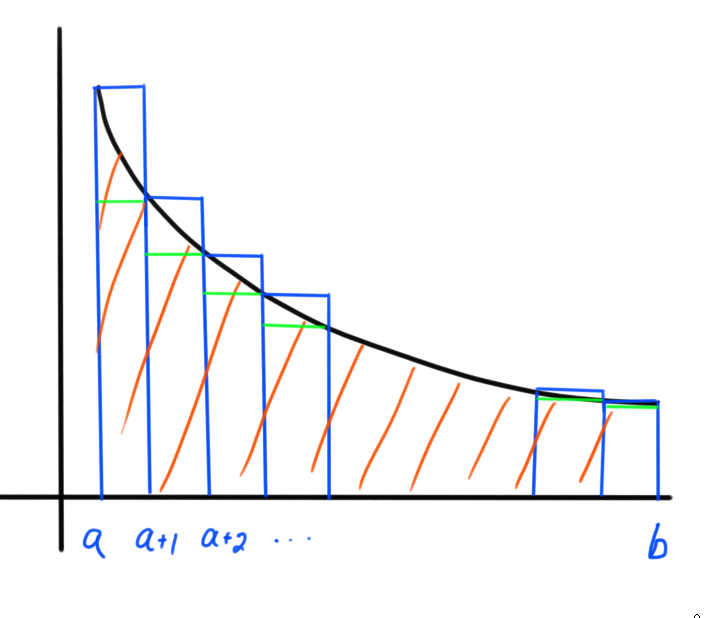
\includegraphics[scale=0.3]{integrals_and_sums}
     \end{figure}
    
    $\sum\limits_{k=a}^b f(k) - \int\limits_a^b \le \sum\limits_{k=a}^b - \sum\limits_{k=a-1}^b = f(a)$ (аналогично $f(b) = \sum\limits_{k=a}^b - \sum\limits_{k=a}^{b-1}$)

\end{proof}
\begin{theorem}[интегральный признак сходимости ряда]
    Пусть $f\!:[1, +\infty) \to \R$ неотрицательная, монотонно убывающая. 

    Тогда  $\sum\limits_{n=1}^\infty f(n)$ и  $\int\limits_1^\infty f(x) \mathrm{d}x$ ведут себя одинаково.
\end{theorem}
\begin{proof}
    По предыдущей теореме $S_n \coloneqq \sum\limits_{k=1}^n f(k) \ge \int\limits_1^n f(x)\mathrm{d}x \ge \sum\limits_{k=2}^n f(k) = S_n - f(1)$.

    Если ряд сходится, то $S_n$ --- ограничена  $\implies \int\limits_1^n f(x)\mathrm{d}x$ ограничена $\implies F(x) = \int\limits_1^x f$ --- ограничена $\implies \int\limits_1^\infty f(x)$ сходится.

    Если  $\int$ сходится $\implies \int\limits_1^n f$ --- ограничена  $\implies S_n$ --- ограничена  $\implies$ ряд сходится.
\end{proof}
\begin{example}
     \begin{enumerate}
         \item $\sum\limits_{n=1}^\infty \frac{1}{n^p}$, $p > 0$ (иначе члены ряда $\centernot \to 0$ и ряд расходится).\\
             $f(x) = \frac{1}{x^p}$. Монотонно убывает. $\sum \frac{1}{n^p}$ и $\int\limits_1^\infty \frac{\mathrm{d}x}{x^p}$ ведут себя одинаково: сходятся при  $p > 1$.
         \item $\sum\limits_{n=2}^\infty \frac{1}{n\ln n}$. $f(x) = \frac{1}{x\ln x}$ монотонно убывает. Поэтому $\int\limits_2^\infty \frac{\mathrm{d}x}{x\ln x}$ и $\sum\limits_{n=2}^\infty \frac{1}{n \ln n}$ ведут себя одинаково. 

             Там можно посчитать интеграл (разойдется).
    \end{enumerate}
\end{example}
\begin{consequence}
    \begin{enumerate}
        \item Если $a_n > 0$ и  $a_n = \mathcal{O}(\frac{1}{n^p})$ при $p > 1$ --- ряд  $\sum a_n$ --- сходится.
        \item Если  $a_n > 0$ и  $a_n \sim \frac{c}{n^p}$, то при $p > 1$ ряд  $\sum a_n$ --- сходится, а иначе расходится.
    \end{enumerate}
\end{consequence}
%END TICKET 59
